\newpage
\section{System Perspective}

%A description and illustration of the:

%  - Design and architecture of your _ITU-MiniTwit_ systems
%  - All dependencies of your _ITU-MiniTwit_ systems on all levels of abstraction and development stages.
%    - That is, list and briefly describe all technologies and tools you applied and depend on.
%  - Important interactions of subsystems
%  - Describe the current state of your systems, for example using results of static analysis and quality assessments.
%  - Finally, describe briefly, if the license that you have chosen for your project is actually compatible with the licenses of all your direct dependencies.

%Double check that for all the weekly tasks (those listed in the schedule) you include the corresponding information.

\subsection{Design and architecture}

The technologies we selected to recreate the legacy flask application ITU-MiniTwit, were C\# with the ASP.NET Core framework for the server and Postgresql as the database. The decision to use ASP.NET Core was made based on the team's prior experience, which enabled us to implement the legacy Flask application's features quickly. Another reason for our selection is that with the performance enhancements of .NET 7, this is a very well performing framework\footnote{14th in this benchmark: 
\url{https://www.techempower.com/benchmarks/#section=data-r21}}. This can also be seen in our group's solution being one of the tops performing in this chart: \url{http://104.248.134.203/chart.svg}. \\

We used Razor pages to render the web pages on the server side. We also considered creating a single-page application as a frontend, such as with Blazor or React, as this would be the more modern approach. However, we stuck with using Razor pages to replicate the original Flask application as much as possible. Further explanation is given in section \ref{evoref}. \\

\begin{figure}[H]
    \centering
    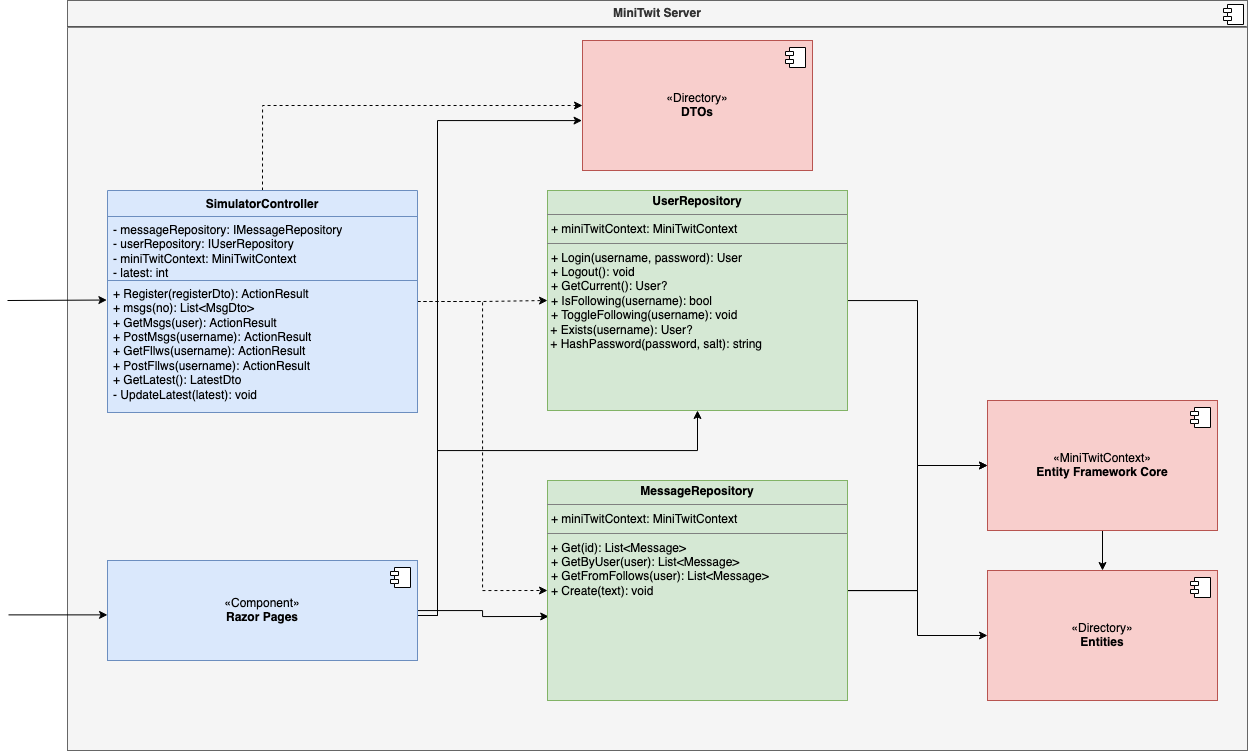
\includegraphics[width=\textwidth]{images/miniTwitServerOverview.png}
    \caption{Architecture of the MiniTwitApi component}
    \label{fig:miniTwitApiOverview}
\end{figure}

For the illustration of the activity on our Minitwit website, we created an API that the simulator could communicate with. Over four weeks, the simulator provided our system with over 4 million messages/posts and nearly 13 million API calls. \\

Figure \ref{fig:architecture} shows the architecture of the final version of the system that was deployed, using three droplets (virtual machines) on DigitalOcean. Docker containers are within a docker swarm and communicate via the internal overlay network. There are three replicas of the MiniTwit server in the swarm, one on each droplet, to ensure availability. The two worker nodes only contain an instance of the MiniTwit server, while the manager includes load balancing, logging, and monitoring services. We decided to keep all these services on the same node to be accessible on the same IP address. Nginx is used for load balancing between the MiniTwit instances.

The database was hosted as a DigitalOcean-managed database so that it was guaranteed to be reliable. Initially, we managed the Postgres database ourselves. However, one day, it suddenly crashed, which caused approximately 12 hours of downtime. We decided to switch to a managed database in our deployment to avoid worrying about this. Running our \textit{infrastructure.sh} script, which deploys the entire system and provisions the infrastructure on DigitalOcean, will make the database a container in the swarm. Rolling updates are implemented through the docker swarm.

\begin{figure}[H]
    \centering
    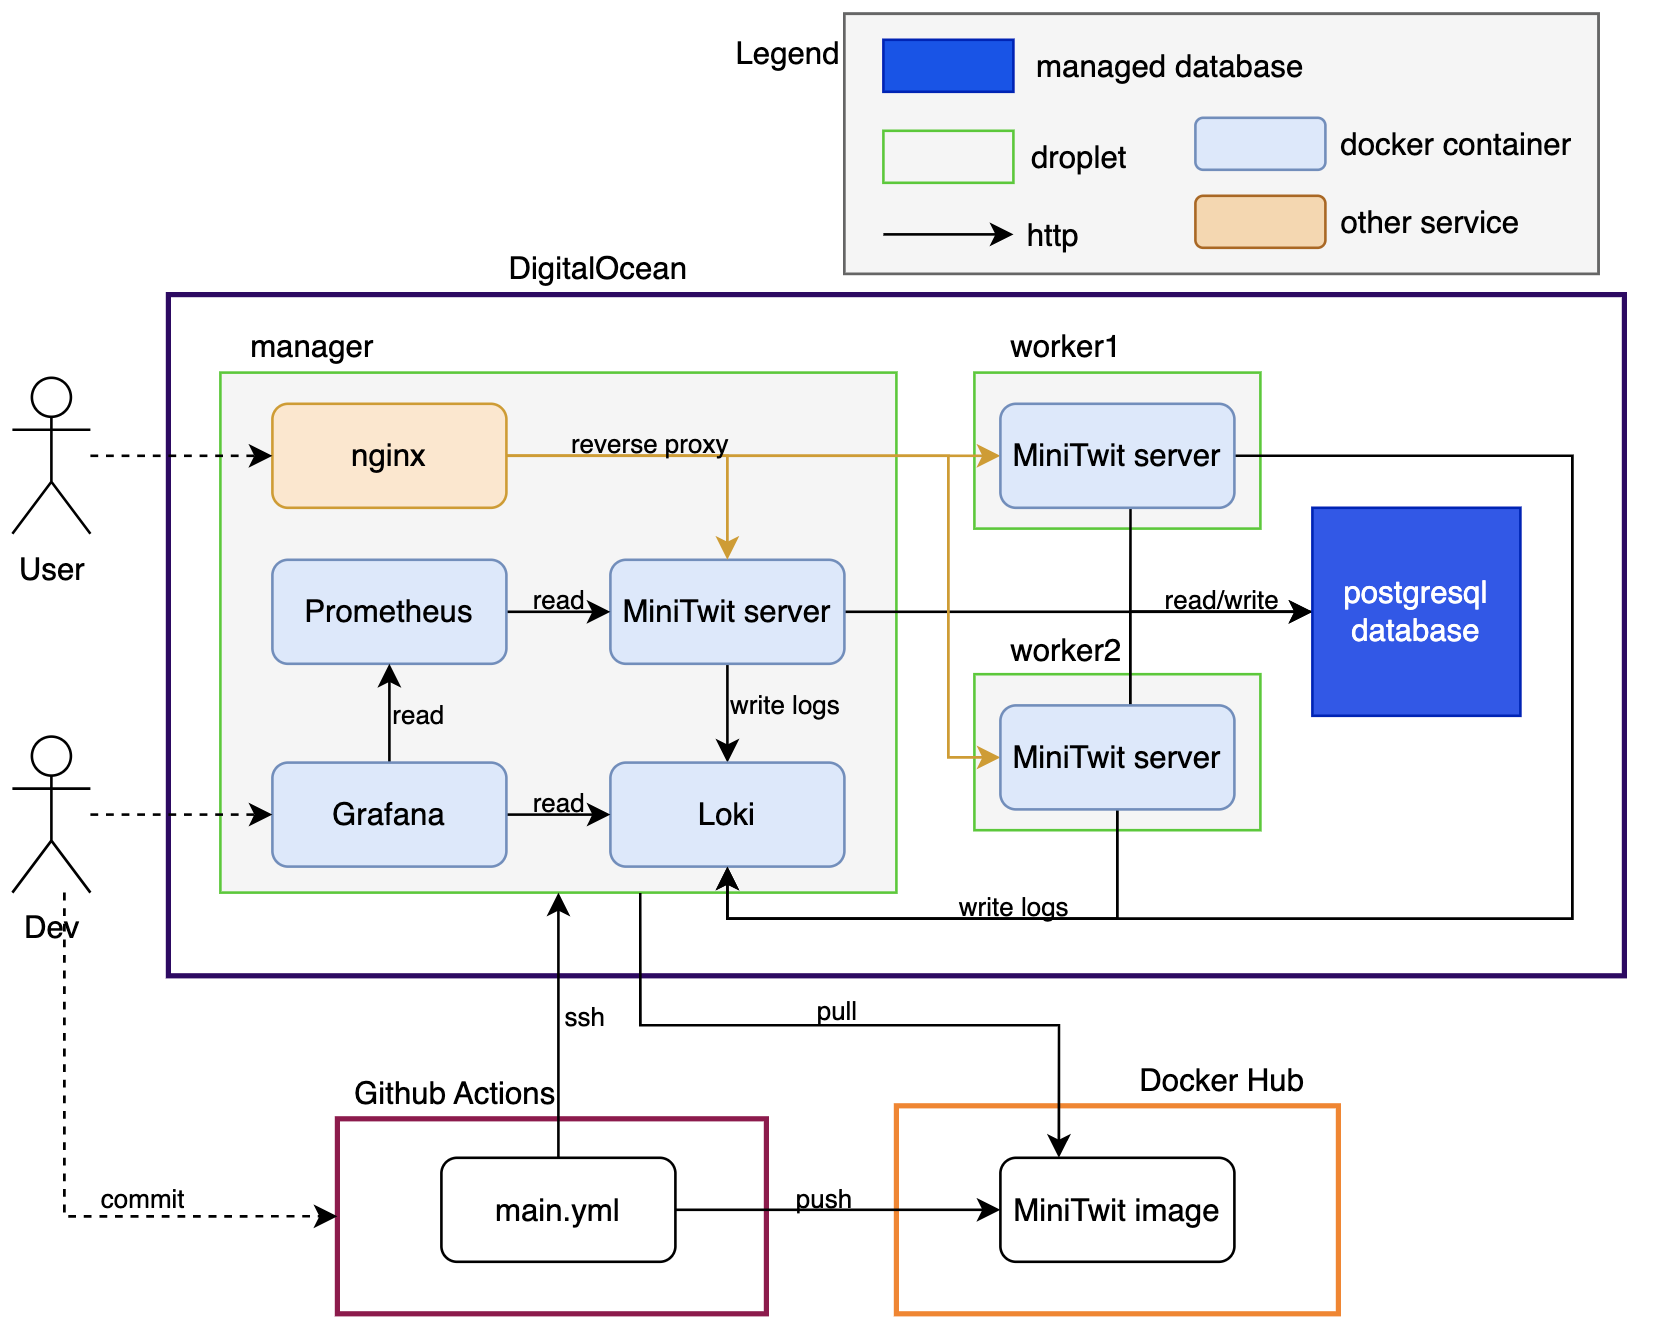
\includegraphics[width=\textwidth]{images/architecture2.png}
    \caption{Architecture of all subsystems in the final system.}
    \label{fig:architecture}
\end{figure}

\subsection{Technologies and Dependencies}

The technologies we have decided on for the system to rely on are listed below. All versions used were the most recent stable releases as of the start of 2023:

\begin{itemize}
    \item \textbf{ASP.NET Core}, for the web application.
    \item \textbf{PostgreSQL}, for data storage.
    \item \textbf{nginx}, for reverse proxy and load balancing.
    \item \textbf{Grafana}, for viewing metrics and logs.
    \item \textbf{Loki}, for storing logs.
    \item \textbf{Prometheus}, for storing metrics.
    \item \textbf{Docker}, for containerization.
    \item \textbf{Docker Hub}, for container image registry.
    \item \textbf{Ubuntu}, for the server OS.
    \item \textbf{Python}, for the tests.
    \item \textbf{Nuget}, for package management.
    \item \textbf{Github Actions}, for CI/CD.
    \item \textbf{DigitalOcean}, for infrastructure.
    \item \textbf{SonarCloud}, for static analysis.
    \item \textbf{Snyk}, for security assessments. \\
\end{itemize}

\noindent The libraries which the ASP.NET Core MiniTwit application depends on are:

\begin{outline}
    \1 \textbf{Entity Framework Core}, library for database abstraction layer.
    \1 \textbf{Npgsql}, library for connecting to Postgres from .NET.
    \1 \textbf{Serilog}, library for logging.
    \1 \textbf{Serilog.Sinks.Grafana.Loki}, library for shipping logs to Loki.
    \1 \textbf{Prometheus-net}, library to instrument .NET code with Prometheus metrics.
    \1 \textbf{SignalR}, library for real-time communication between server and client.
    \1 \textbf{code-cracker}, library for analyzing code.
\end{outline}

\subsection{Important interactions of subsystems}

Figure \ref{fig:architecture} shows the interactions of the subsystems. Docker containers communicate via the internal network within the swarm.

When a developer pushes to the main branch on GitHub, the \textit{main.yml} workflow is run. First, the system is built on the workflow server via Docker-Compose, then the Python tests interact with the system via HTTP. We have refactored and expanded the Python tests from the exercises. If the tests all pass, the workflow pushes the new MiniTwit image to Docker Hub. It then utilizes ssh to execute a script on the manager node, which pulls the image and updates the workers. Finally, a GitHub release is created by the workflow.

A shortcoming of our chosen architecture is that Prometheus only reads from one of the MiniTwit server instances, the one on the same node. Since the load is balanced, only 33\% of the traffic is monitored by metrics. This is not optimal since it does not give all of the information. However, it presents a snippet of the system's monitoring. The same problem appeared with the real-time updates implemented with SignalR. Because of the load balancing, only every third message will, on average, appear for the user without reloading the page.

\subsection{Current state of systems}
Due to our project utilizing infrastructure as code, it is possible to turn the system on/off quickly. When writing this report, we have turned the system off to minimize payments to Digital Ocean. When turning our system on, everything works as expected. However, there is little to no traffic since the simulator has stopped. The current code quality can be seen on our SonarQube page, which is showcased in figure \ref{fig:sonarQubeOverview}.

\begin{figure}[H]
    \centering
    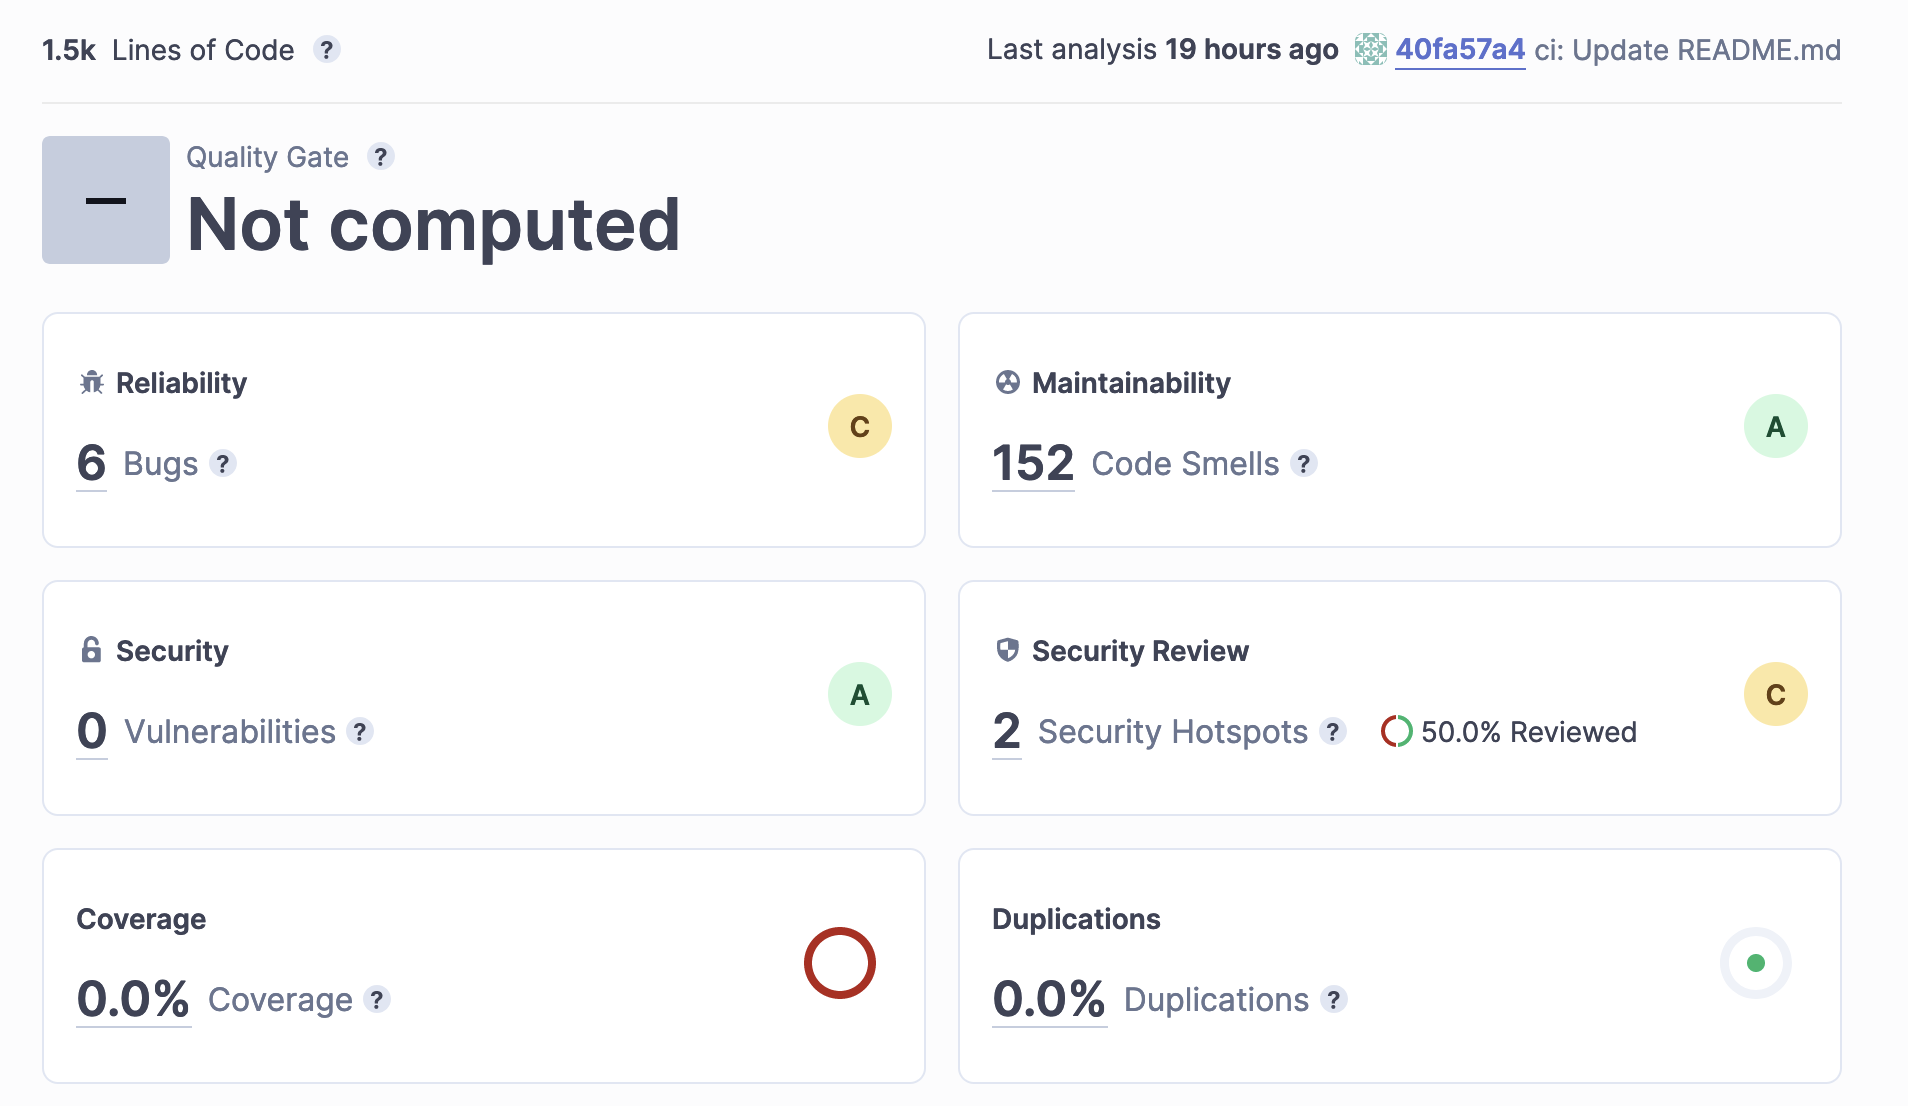
\includegraphics[width=\textwidth]{images/sonarStats.png}
    \caption{An overview of the code quality of the project in SonarQube.}
    \label{fig:sonarQubeOverview}
\end{figure}

%\todo[inline]{her kunne man lave sådan noget future work, altså hvis vi skulle arbejde videre på det hvad ville vi så lave?}

For future work on the project, it would make sense to perfect the load-balancing aspect of the dockerized swarm. For example, the current setup means that Grafana only shows 1/3 of metrics, and when a user is connected to a MiniTwit server via WebSockets, this user would only receive 1/3 of new tweets. Currently, the WebSockets only send messages to clients when a change happens on the server instance, not when a change occurs in the database.

\subsection{License of our systems}
As we use the MIT license, and most of the direct dependencies use AGPLV3, we do not have any license conflicts. Our API also has an SLA.